\section{Q6 — Cross-Variable Forecast Error Correlations}


\textbf{Research question:}

\begin{quote}
How are forecast errors correlated across weather variables, and which variables tend to have related forecast-error behavior?
\end{quote}

\subsection{Data and Method}

Forecast errors from the December 30 and December 31 forecast cycles were combined across all available sites. Before computing correlations, duplicate observations were grouped by site ID and valid time, and the mean error was used for each site-time pair. This produced 23,505,664 aligned site-time observations across 896 sites.

For each pair of weather variables, the Pearson correlation coefficient was computed between their forecast-error time series. Only rows where both error values were finite were included. The resulting Pearson value measures the linear relationship between two forecast errors:

\[
r = \frac{\mathrm{cov}(X,Y)}{\sigma_X \sigma_Y}.
\]

A positive value means that the two forecast errors tend to increase or decrease together. A negative value means that one error tends to increase when the other decreases. A value near zero means that there is little linear relationship between the two error series.

\subsection{Pairwise Error Correlation Heatmap}

The pairwise correlation heatmap summarizes the Pearson correlation values across all weather-variable error pairs. Blue cells represent negative correlations, red cells represent positive correlations, and lighter cells represent correlations closer to zero.

\begin{figure}[H]
    \centering
    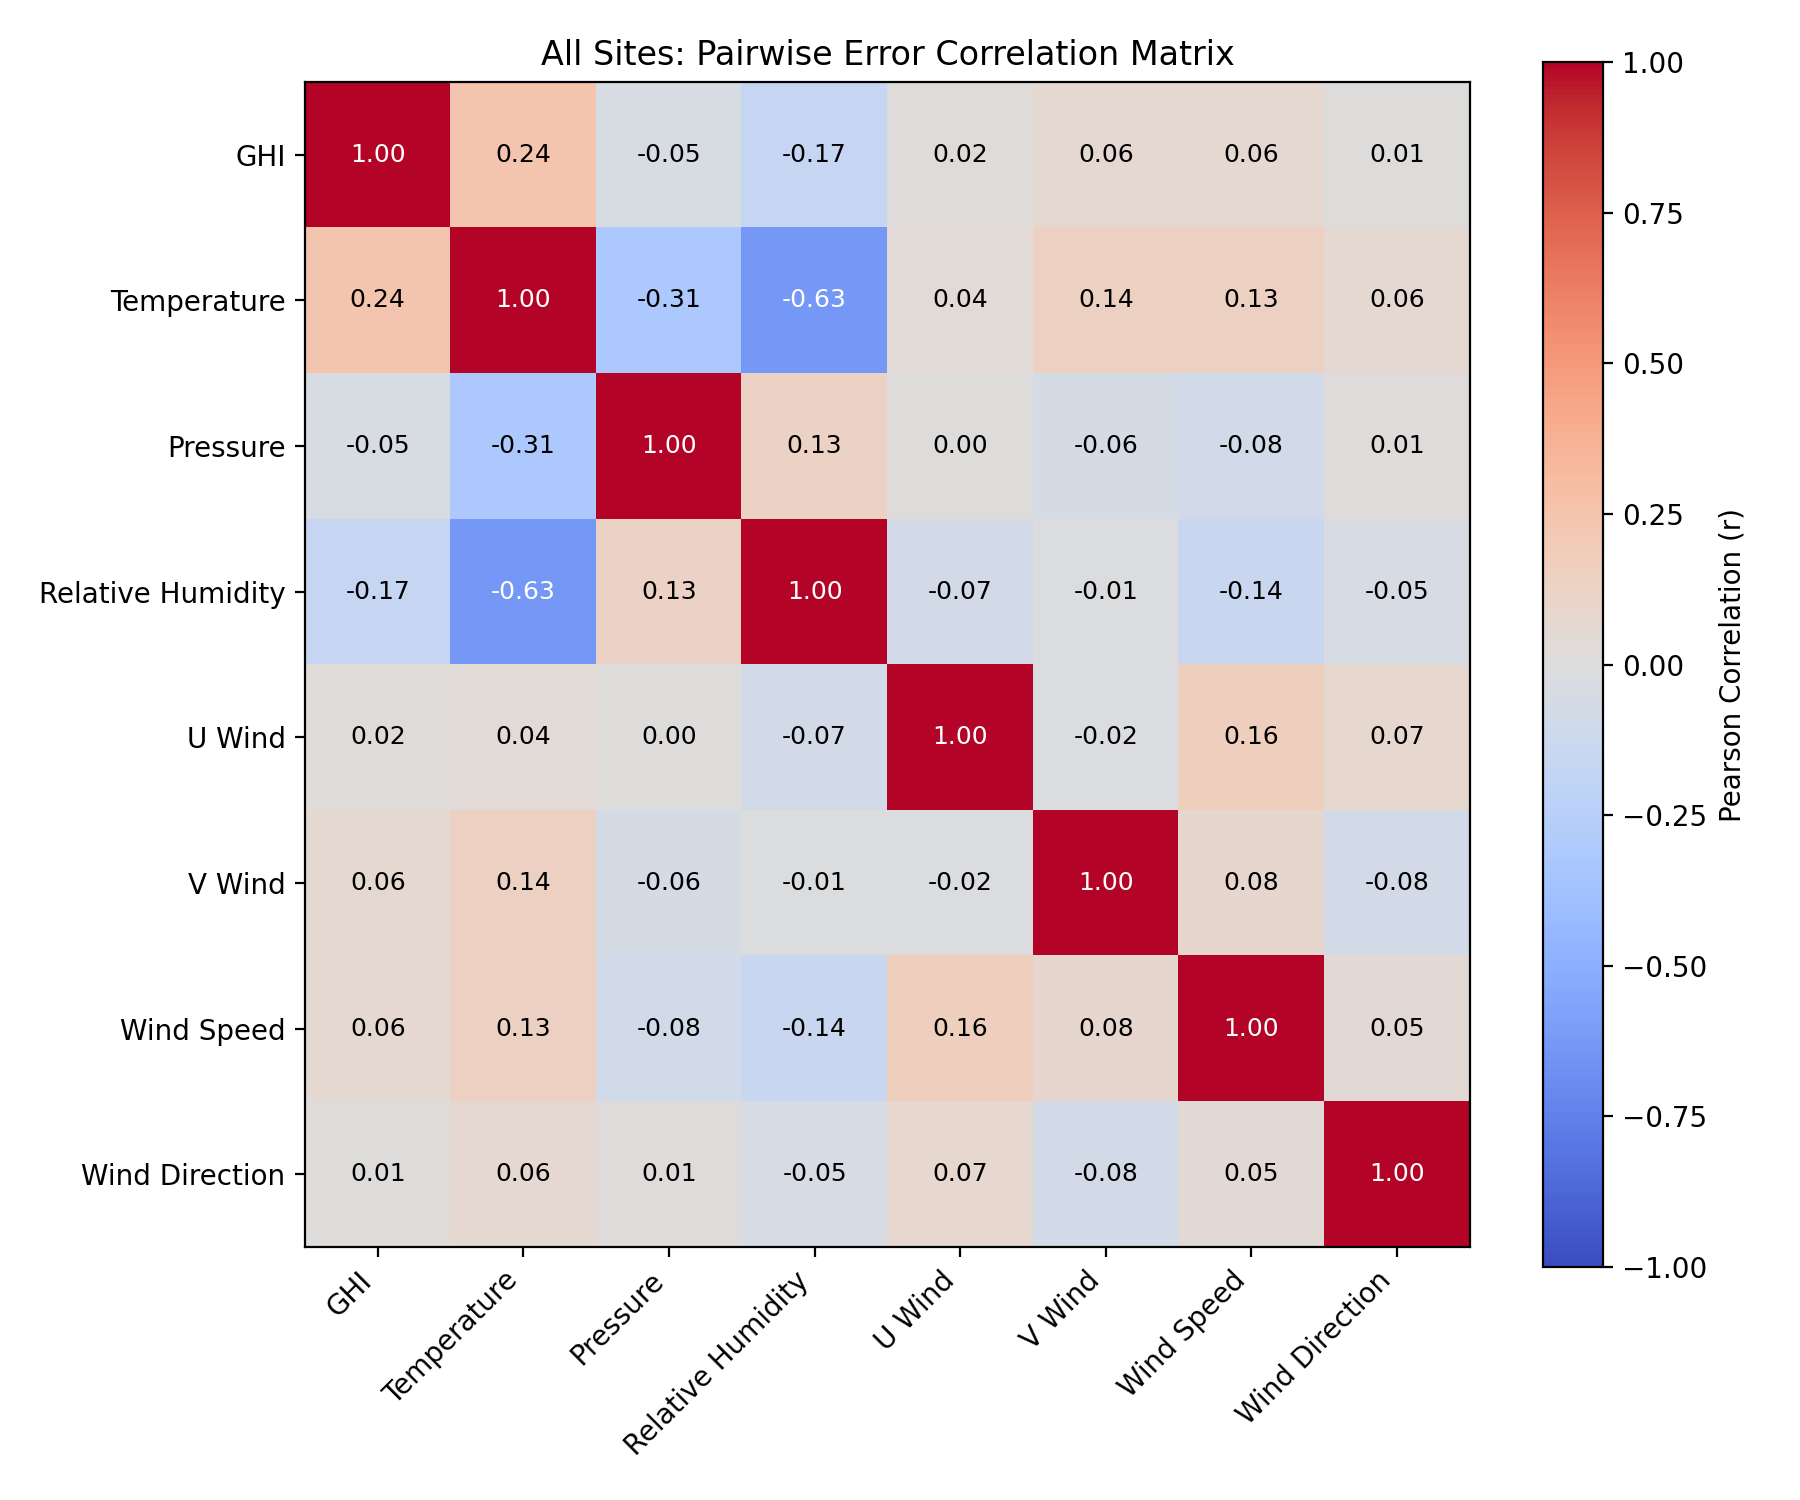
\includegraphics[width=0.65\textwidth]{figures/Q6/allsites_pairwise_error_correlation_matrix.png}
    \caption{Pairwise Pearson correlations between forecast-error variables across all sites and valid times.}
    \label{fig:q6_pairwise_error_correlation}
\end{figure}

\subsection{Main Correlation Patterns}

The strongest cross-variable relationship is between temperature error and relative humidity error, with a Pearson correlation of approximately $r=-0.626$. This negative relationship means that positive temperature forecast errors tend to occur with negative relative-humidity forecast errors, and vice versa. This is physically reasonable because temperature and relative humidity are closely connected through atmospheric moisture capacity.

Temperature error also has a moderate negative relationship with pressure error, with $r=-0.313$, and a weaker positive relationship with GHI error, with $r=0.238$. These values suggest that temperature-error behavior is more connected to other thermodynamic and radiation-related errors than to wind errors.

Most wind-variable relationships are comparatively weak. U wind and V wind have a correlation close to zero, $r=-0.023$, and their relationships with wind speed are also weak: U wind vs. wind speed has $r=0.163$, while V wind vs. wind speed has $r=0.081$. This does not mean that wind components are physically unrelated to wind speed. Instead, it reflects that this analysis compares forecast errors, not the raw meteorological variables. Because U and V wind are signed directional components while wind speed is a nonnegative magnitude, their signed errors can cancel out across many wind directions, sites, and times.

\subsection{Interpretation}

The correlation matrix shows that cross-variable forecast-error dependence is strongest among temperature, relative humidity, pressure, and GHI. The strongest relationship is the negative temperature--relative humidity error correlation. Pressure and GHI also show some relationship with temperature, but the correlations are weaker.

Wind direction and the wind components show relatively low correlations with most other variables. This suggests that wind forecast errors are less linearly connected to the thermodynamic and radiation variables in this pooled all-site analysis. It may also indicate that wind errors depend more strongly on local flow, terrain, and direction-specific behavior than on the broad atmospheric relationships captured by a simple Pearson correlation.

\subsection{Conclusion}

Forecast errors are not independent across all weather variables. The clearest cross-variable dependence occurs between temperature and relative humidity errors, followed by weaker relationships involving pressure, GHI, and temperature. Wind-related forecast errors are much less correlated with the other variables in the all-site Pearson correlation matrix. Overall, the Q6 results suggest that thermodynamic and radiation-related forecast errors share more common structure, while wind-variable errors behave more independently in this analysis.
